\documentclass{article}
\usepackage{tikz}
\usetikzlibrary{shapes.geometric}

\begin{document}

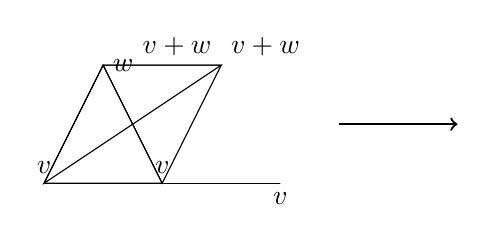
\begin{tikzpicture}[scale=1.5]
    % Define the vertices of the first triangle
    \coordinate (A) at (0,0);
    \coordinate (B) at (1,0);
    \coordinate (C) at (0.5,1);

    % Draw the first triangle
    \draw (A) -- (B) -- (C) -- cycle;

    % Label the vertices with 'v' and 'w'
    \node at (A) [above] {$v$};
    \node at (B) [above] {$v$};
    \node at (C) [right] {$w$};

    % Draw the second triangle
    \draw (B) -- (C) -- ++(1,0) coordinate (D) -- cycle;
    \draw (A) -- (C) -- ++(1,0) coordinate (E) -- cycle;
    \draw (A) -- (B) -- ++(1,0) coordinate (F) -- cycle;

    % Label the new vertices with 'v+w' and 'v'
    \node at (D) [above right] {$v+w$};
    \node at (E) [above left] {$v+w$};
    \node at (F) [below] {$v$};

    % Add an arrow indicating the transformation
    \draw[->, thick] (2.5,0.5) -- (3.5,0.5);
\end{tikzpicture}

\end{document}